\setcounter{equation}{0}
\chapter{Discussion}
\label{chap:discussion}

\section{Comparison with an observation}

There are several observations of LAEs in the literature. One that records the spectra of a distant LAE ($z\sim2.1974$) and has high resolution is published by Kulas et al. \cite{Kulas12}. In the Figure 3 of their paper \ref{fig:kulas} they show 18 different \lya profiles. \\

\begin{figure}[h!]
	\begin{center}
		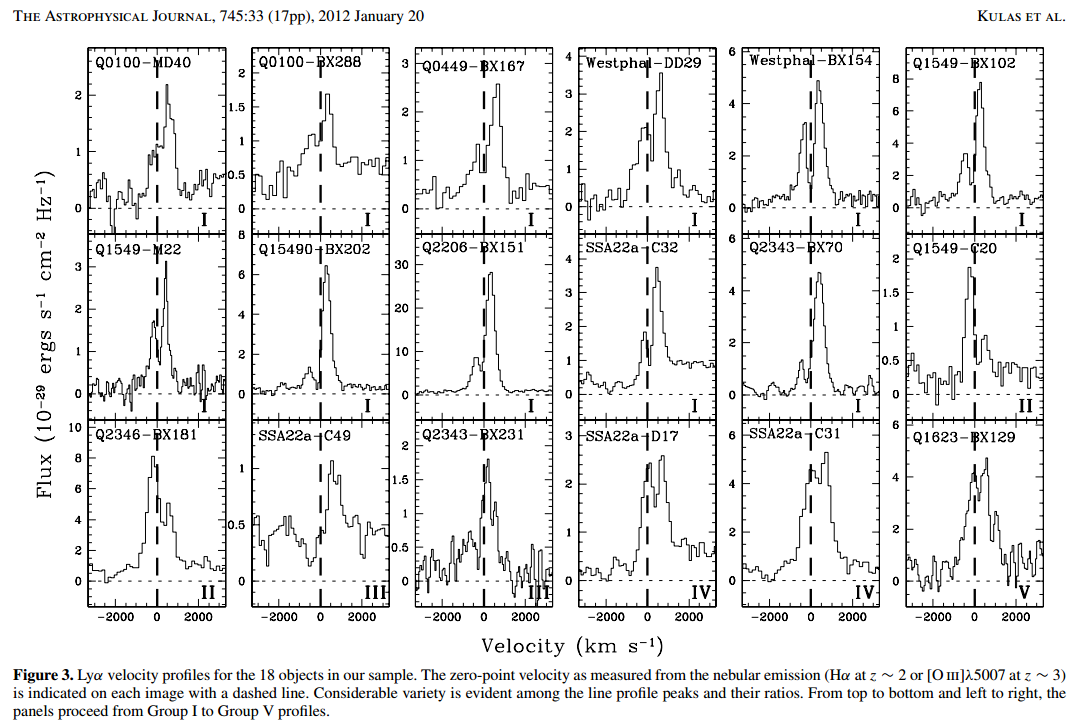
\includegraphics[width=1\textwidth]{./figures/chapter4/figure3}
	\end{center}
	\caption{\textbf{Figure 3 of Kulas et al. paper} \cite{Kulas12}
		\label{fig:kulas}}
\end{figure}
%http://arohatgi.info/WebPlotDigitizer/app/

In the x axis of these spectra they used the variable velocity. It is another way to represent the photon's wavelength. However, this new variable has units. Also, now the photon is redshifted in frequency is when the velocity is greater than 0. The blueshift is the opposite. For this reason they seem reflexed around the y axis. \\

Besides this reflection, the observed spectra in Fig. \ref{fig:kulas} is also modified by the redshift of the galaxies. This is, how much distance light had to travel to reach their telescopes. That causes a broadening of the line. \\

Without taking into account these two effects, one can notice a clear similitude between them and my simulated ones. The \lya profiles are mostly 2 peaks with an asymmetry between them, just as in the simulation. Also, the small peak (if existing) is always a lot smaller than the tall one.\\

\section{Importance of this result}

The main result of this monograph is that I achieved a LAE model consistent with observations that nobody has done before.\\

Many authors that only include the outflows effect are able to fit observational spectra but with a very large magnitude of \vout. It is important to recall that \vout is caused mainly by ejection of material out the galaxy. It is then common that a galaxy rotates faster than it expands, not the opposite. \\

And others that include the rotational effect are able to obtain the two peaks but not their asymmetry. This only emulates LAEs without outflows. So, the model does not replicate the majority of the cases. \\

The combination of rotation and outflows velocities not only makes a lot of sense but fits really well to observations. Also, the new model proposed in this monograph can replicate \lya profiles with typical LAE's values.\\


\section{Future work}

\subsection{Non-central emission}
As mentioned in Chapter \ref{chap:model}, the initial emission of each photon always begins in th center of the galaxy. For this, it would be interesting to run the same simulation but with an emission distributed uniformly around the sphere. \\

This non-central emission could improve the accuracy of the model by approaching a more realistic light emission. However, the results are obtained and compared to conclude this. \\

\subsection{Parameter fit of an observation}
Due to the long time CLARA takes to run, it was not possible in this work to made a fit of an observational \lya and predict its parameters. However, with more time, it would be really interesting to use tools as MCMC (Monte Carlo Markov Chain) to obtain the observed galaxy's \tauh, \vrot and \vout that would agree with my model. \\